\section{Dynamics in an Asymmetric Hamiltonian} \label{sec:asymham}

The previous section, and much of the current literature, focuses on symmetric Hamiltonian systems, in that the butterfly velocity is the same for perturbations traveling to the left or to the right. Ref.\cite{??} mentions...

In this section we study the operator dynamics of an asymmetric time-independent Hamiltonian system. First we construct the local 3-site Hamiltonian through its action on the computational basis. 
After chaining together these local terms to define a multi-site Hamiltonian we find the behavior of the Pauli weights and OTOC. Eventually we show that this system has two distinct butterfly velocities, one for operator fronts spreading in each direction.

\subsection{3-Site Hamiltonian}  \label{sub:hamiltonian}

We want a multi-site in which sites interact only through local interactions. We can accomplish this by defining an $n$-site Hamiltonian for $n$ small, and then putting this Hamiltonian on each set of $n$ sites,
\begin{align}
H_{\text{tot}} = \sum_{i=0}^{L-n}H_n^{(i)},
 \label{eqn:chain}
\end{align}
where $H_n^{(i)}$ is a $n$-site Hamiltonian acting on sites $i$ through $i+n-1$.
A common choice is $n=2$ but this will not suffice, because 2-site Hamiltonians are always symmetric with respect to their operator dynamics. Unitarity preserves information so for any weight the 2-site Hamiltonian moves from site $i$ to $i+1$ it must move an equal amount from site $i+1$ to $i$. 3-site Hamiltonian do not have this constraint, though, and can have asymmetric dynamics.

The feature we are looking for in this Hamiltonian is asymmetry in its dynamics. To that end, instead of looking directly for an asymmetric Hamiltonian, we can find a unitary operator $U(t)$ with the dynamics we want. From that operator we can construct a Hamiltonian that gives $U(t)=e^{-iHt}$. There are multiple ways to construct $H$ from $U(T)$. One way is to just take the matrix log, for example by using Mathematica. Since this method is not very physical, we can instead look at eigenstates. $U(t)$ and $H$ will have the same eigenstates, with the eigenvalues of $H$ given by $\lambda_H = i\log(U(1))$. The Hamiltonian is completely specified by its eigenstates and eigenvalues. Since scalar logs are easier, this method is much more intuitive.

One asymmetric unitary operator is the 3-site cyclic swap $S_{123}$. $S_{123}$ is a unitary operator such that
\begin{align}
S_{123}\ket{\alpha\beta\gamma} =\ket{\gamma\alpha\beta}, \label{eqn:condition}
\end{align}
where $\ket{\alpha\beta\gamma}$ is a product state with state $\ket{\alpha}$ on site 0, $\ket{\beta}$ on site 1, and $\ket{\gamma}$ on site 2. The idea of using this operator is that it can transport a state from site 3 to site 1 in 1 step, but takes two applications to move a state from site 1 to site 3.

One way to build the three site swap gate is in a Floquet system or quantum circuit, out of 2-site swap gates $S_{123} = S_{12}S_{23}$. Each 2-site swap interchanges two states, so the action is 
\begin{align}
S_{12}S_{23}\ket{\alpha\beta\gamma} &= S_{12}\ket{\alpha\gamma\beta} = 
	\ket{\gamma\alpha\beta}\nn
&= S_{123}\ket{\alpha\beta\gamma}.
\end{align}
It is also possible to build $S_{123}$t out of a time-independent Hamiltonian, so that $U(t=1) = e^{-iH_3} = S_{123}$. We will construct the Hamiltonian using the eigendecomposition, but it is also possible to take the matrix log.

For a system with spin-$\half$ objects on the sites there is an 8-dimensional Hilbert space, which can be decomposed into a spin-$\frac{3}{2}$ subspace with 4 states and 2 spin-$\half$ subspaces with 2 states each. Since the eigenstates of $S_{123}$ only pick up a phase under unitary evolution, they will be states in which individual particle states differ only by phases, so that the phase from the dynamics effectively permutes the states. 

There are four states that are symmetric with respect to the three sites, and therefore should not change in time and have 0 energy. Before normalization these are
\begin{align}
\ket{\psi_{0,0}}=\ket{000},\quad \ket{\psi_{0,1}}=\ket{100}+\ket{010}+\ket{001},
	\nn
\ket{\psi_{0,3}}=\ket{111},\quad \ket{\psi_{0,2}}=\ket{011}+\ket{101}+\ket{110},
	\label{eqn:zero}
\end{align}
where, for example, $\ket{001}$ is a product state with sites 0 and 1 in state $\ket{0}$ and site 3 in state $\ket{1}$. $\ket{1}$ is the spin-up state and $\ket{0}$ is the spin-down state.

Of the four other states, two should have positive energy and two should have negative energy. Since $U(t=3)=1$, their eigenvalues must be cube roots of unity. The energies should be $E_\pm = \pm\frac{2\pi}{3}$ so they pick up a phase $\phi_\pm =e^{-iE_\pm} = e^{\mp i\frac{2\pi}{3}}$. Using condition~\ref{eqn:condition}, we can show that the positive energy states are
\begin{align}
\ket{\psi_{+,1}}=&\ket{100} + \phi_-\ket{010} + \phi_+\ket{001},\nn
\ket{\psi_{+,2}}=&\ket{011} + \phi_-\ket{101} + \phi_+\ket{110},\label{eqn:plus}
\end{align}
while the negative energy states are 
\begin{align}
\ket{\psi_{-,1}}=&\ket{100} + \phi_+\ket{010} + \phi_-\ket{001},\nn
\ket{\psi_{-,2}}=&\ket{011} + \phi_+\ket{101} + \phi_-\ket{110}.\label{eqn:min}
\end{align}
For example. the evolution of $\ket{\psi_{+,1}}$ is
\begin{align}
U(1)\ket{\psi_{+,1}} &= \phi_+ \left(\ket{100} + \phi_-\ket{010} + \phi_+
	\ket{001}\right)\nn
&= \phi_+\ket{100} + \ket{010} +\phi_- \ket{001}\nn
&= S_{123}\ket{\psi_{+,1}},
\end{align}
with similar results for the other 3 non-zero energy states.

To write the Hamiltonian as a matrix we have to choose a basis. In the eigenbasis, of course, the Hamiltonian is diagonal. A more useful basis is the computational basis, which has states $\ket{000},\,\ket{001},\,\ket{010},\,\ket{011},\,\ket{100},\,\ket{101},\,\ket{110},\,\ket{111}$. The strings inside each ket can be interpreted as binary number, so that the states can be written as $\ket{0},\,\ket{1},\,\ket{2}$, etc.

Then the Hamiltonian is 
\begin{align}
H_3 = T\; \text{diag}(0,0,0,0,E_+,E_+,E_-,E_-)\; T^\dag,
\end{align}
where diag(\dots) is the Hamiltonian in its eigenbasis and $T$ is the transformation matrix between the two bases, which can be found from the form of the 3 eigenstates in Eqs.~\ref{eqn:zero}, \ref{eqn:plus}, and~\ref{eqn:min},
\begin{align}
T = \th{\sqrt{3}}\begin{bmatrix}
\sqrt{3} & 0 & 0 & 0        & 0      & 0      & 0      & 0      \\
0        & 1 & 0 & 0        & \phi_+ & 0      & \phi_- & 0      \\
0        & 1 & 0 & 0        & \phi_- & 0      & \phi_+ & 0      \\
0        & 0 & 1 & 0        & 0      & 1      & 0      & 1      \\
0        & 1 & 0 & 0        & 1      & 0      & 1      & 0      \\
0        & 0 & 1 & 0        & 0      & \phi_- & 0      & \phi_+ \\
0        & 0 & 1 & 0        & 0      & \phi_+ & 0      & \phi_- \\
0        & 0 & 0 & \sqrt{3} & 0      & 0      & 0      & 0
\end{bmatrix}
\end{align}
Altogether, the Hamiltonian is
\begin{align}
H_3 = \frac{2\pi i}{3\sqrt{3}}\begin{bmatrix}
0 & 0  & 0  & 0  & 0  & 0  & 0  & 0 \\
0 & 0  & 1  & 0  & -1 & 0  & 0  & 0 \\
0 & -1 & 0  & 0  & 1  & 0  & 0  & 0 \\
0 & 0  & 0  & 0  & 0  & -1 & 1  & 0 \\
0 & 1  & -1 & 0  & 0  & 0  & 0  & 0 \\
0 & 0  & 0  & 1  & 0  & 0  & -1 & 0 \\
0 & 0  & 0  & -1 & 0  & 1  & 0  & 0 \\
0 & 0  & 0  & 0  & 0  & 0  & 0  & 0 \\
\end{bmatrix}\label{eqn:3ham}
\end{align}

This Hamiltonian is antisymmetric and purely imaginary. One effect of this is that if the system starts in a state with real coefficients all coefficients stay real because
\begin{align}
\dot{\psi}=-iH\psi
\end{align}
is purely real.
Before moving on we note that this commutes with the total spin-Z operator 
\begin{align}
S_Z = \text{diag}\left(-\frac{3}{2}, -\frac{1}{2}, -\frac{1}{2}, \frac{1}{2}, -\frac{1}{2}, \frac{1}{2}, \frac{1}{2}, \frac{3}{2}\right)
\end{align}
so total spin-Z is conserved. It also commutes with the other components of spin and therefore also total spin $S^2$.

There are a few checks we can perform on this Hamiltonian, First, it should be symmetric under a simultaneous rotation of all three spins in real space, so that it can be written as $H_3(\bm{S}_1,\,\bm{S}_2 ,\,\bm{S}_3)$ as a function invariant to simultaneous rotations of the three spin vectors. Furthermore it should be antisymmetric under the interchange of any two spins (equivalent to reversing the direction of propagation). The only function of three vectors that has this property is the triple product $H_3= \bm{S}_1\cdot\left(\bm{S}_2 \times\bm{S}_3\right)$, where multiplication of components is interpreted as tensor products.

The representation of the Hamiltonian as a triple product provides another reason for the spectrum of the Hamiltonian. As previously mentioned the Hilbert space of the 3 spins decomposes into one spin-$\frac{3}{2}$ space and two spin-$\half$ spaces. The state $\ket{111}$ is part of the spin-$\frac{3}{2}$ space. Since the three spins point in the same direction, their triple product vanished. Furthermore, since the other three states in the spin-$\frac{3}{2}$ subspace are related to $\ket{111}$ by rotation and the Hamiltonian is symmetric in this respect they also must have energy 0. Of the two spin-$\half$ pairs, one pair has positive energy and one has negative energy.

Writing the $j$th component of spin on site $i$ as $S_{i,j}$, this triple product is
\begin{align}
H &= \bm{S}_1\cdot\left(\bm{S}_2 \times\bm{S}_3\right) \nn
&= S_{1,1}\otimes S_{2,2}\otimes{S}_{3,3} - {S}_{1,1}
	\otimes S_{2,3}\otimes S_{3,2} + S_{1,2}\otimes{S}_{2,3} \otimes {S}_{3,1}-\cdots\nn
&= \begin{bmatrix}
	0 & 0 & 0 & 0 & 0 & 0 &-i & 0 \\
	0 & 0 & 0 & 0 & 0 & 0 & 0 & i \\
	0 & 0 & 0 & 0 &-i & 0 & 0 & 0 \\
	0 & 0 & 0 & 0 & 0 & i & 0 & 0 \\
	0 & 0 &-i & 0 & 0 & 0 & 0 & 0 \\
	0 & 0 & 0 & i & 0 & 0 & 0 & 0 \\
	-i& 0 & 0 & 0 & 0 & 0 & 0 & 0 \\
	0 & i & 0 & 0 & 0 & 0 & 0 & 0
	\end{bmatrix} + \dots
\end{align}
which the reader can check is indeed proportional to Eq.~\ref{eqn:3ham}.

Exponentiating the Hamiltonian should act as another check. This gives the time evolution operator for one time step
\begin{align}
U(t=1) = e^{-iH_3} = \begin{bmatrix}
1 & 0 & 0 & 0 & 0 & 0 & 0 & 0 \\
0 & 0 & 1 & 0 & 0 & 0 & 0 & 0 \\
0 & 0 & 0 & 0 & 1 & 0 & 0 & 0 \\
0 & 0 & 0 & 0 & 0 & 0 & 1 & 0 \\
0 & 1 & 0 & 0 & 0 & 0 & 0 & 0 \\
0 & 0 & 0 & 1 & 0 & 0 & 0 & 0 \\
0 & 0 & 0 & 0 & 0 & 1 & 0 & 0 \\
0 & 0 & 0 & 0 & 0 & 0 & 0 & 1
\end{bmatrix}
\end{align}
This has the properties of of condition~\ref{eqn:condition}. Furthermore, application three times gives $U(t=3) = 1$. 

We can learn more about this Hamiltonian by watching the evolution of a single state. If the system starts in the state $\ket{100}$, the coefficients for the other states with equal total $S_Z$ will both change from 0 while the other coefficients will stay 0 due to conservation of $S_Z$. Furthermore we know that the coefficients should remain real, so we can plot the actual coefficients instead of their magnitudes.
From the definition of the unitary operator we know the state will become $\ket{010}$ at time 1. Fig.~\ref{fig:timeevol} shows this evolution. An important point to realize is that the coefficient of $\ket{001}$ also becomes non-zero at early time, as it must for evolution under a time-independent Hamiltonian if it is going to become non-zero in the future. In fact, at early time the coefficients for $\ket{010}$ and $\ket{001}$ increase with the same magnitude.
\begin{figure}
	\centering
	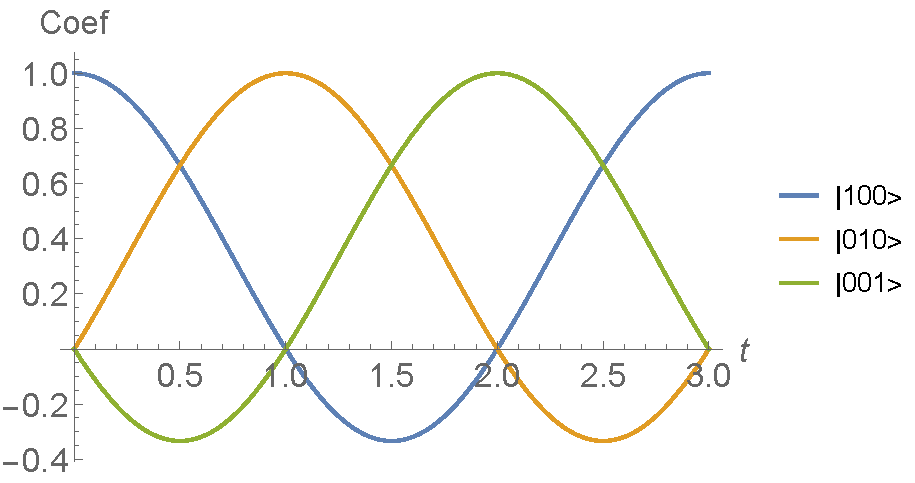
\includegraphics[width=.5\textwidth]{timeevol}
	\caption{\textbf{Evolution of coefficients in 3-site system} if the system starts in state $\ket{100}$. Note that the system initially moves to states $\ket{010}$ and $\ket{001}$ with equal coefficient squared, although at time $t=1$ the state is entirely $\ket{010}$.}
	\label{fig:timeevol}
\end{figure}

\subsection{Multi-Site Hamiltonian} \label{sub:multistate}

The 3-site system is periodic, and furthermore is not large enough to effectively study operator spreading. One way would be to apply $H_3$ repeatedly to each triplet of spins. This would equivalently apply $S_{123}$ to each triplet. However this is not a time-independent Hamiltonian, but rather a Floquet system. To preserve time independence we can apply the 3-site Hamiltonian to all triplets simultaneously, as in Eqn.~\ref{eqn:chain}. Note that this means that $U(t)$ will no longer simply shuffle the states as in  Eqn.~\ref{eqn:condition}. This subsection will explore the dynamics of this multi-site Hamiltonian.

Since the perturbations on states move from site $0\to1\to2\to0$, after chaining multiple Hamiltonians together the perturbations should move faster from high $i$ to low $i$, which we will call the backward direction. Heuristically, this is because weight can ``jump" directly from site 2 to site 0, but has to move through site 1 when it is moving forward. Once we get to the butterfly velocity, which is defined in terms of perturbations to operators, we expect the velocity to be faster forward, since operators evolve in the opposite direction from states.

\subsubsection{Construction} \label{subsub:construction} 

Explicitly, the extension of this Hamiltonian to 4 sites is, using the notation in Eq.~\ref{eqn:chain},
\begin{align}
H_4 = H_3^{(0)}\otimes\mathbb{I}_1^{(3)} + \mathbb{I}_1^{(0)}\otimes H_3^{(1)},
\end{align}
so that the 3-site Hamiltonian acts on each contiguous triplet of spins.
This Hamiltonian still preserves each component of total spin. Since we are applying the Hamiltonian to the 4 sites simultaneous, its unitary behavior does not simply swap states between the sites. However, the behavior is still periodic. Fig.~\ref{fig:timeevol4} shows that when the system starts in state $\ket{0001}$ it returns to that state with period $\tau=3\sqrt{\frac{3}{5}}$ but never fully reaches any other basis state.
\begin{figure}
\centering
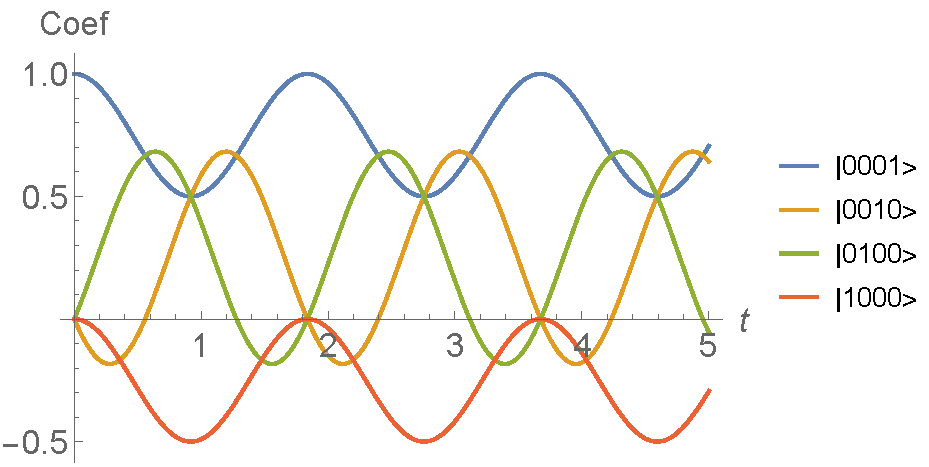
\includegraphics[width=.5\linewidth]{timeevol4}
\caption{\textbf{Evolution of the 4-site system} when the initial state is $\ket{0001}$. Each curve is the coefficient of one of the basis states. The system is periodic with period $\tau=3\sqrt{\frac{3}{5}}$, and is never fully in one of the other basis states.}
\label{fig:timeevol4}
\end{figure}

With 5 sites, adding the third triplet destroys the simple periodic behavior of the system, although it is still quasiperiodic. The Hamiltonian is now
\begin{align}
H_5 = H_3^{(0)}\otimes\mathbb{I}^{(3)}\otimes\mathbb{I}^{(4)} + 
	\mathbb{I}^{(0)}\otimes H_3^{(1)}\otimes\mathbb{I}^{(4)} +
	\mathbb{I}^{(0)}\otimes\mathbb{I}^{(1)}\otimes H_3^{(2)},
\end{align} 
so that there is again one 3-site Hamiltonian on each contiguous triplet.
Starting in $\ket{00001}$, the coefficients follow the pattern of figure~\ref{fig:timeevol5}. At first the evolution is similar to the $n=1$ case, with $\ket{10000}$ and then $\ket{01000}$ reaching near maximal. This suggests that the system retains some of its swap gate-like behavior. However the system is never fully in any basis state after $t=0$, due to the lack of periodicity.

By directly diagonalizing the Hamiltonian we can study the evolution of a single component of the state. The coefficient of $\ket{00001}$ is 
\begin{align}
c_1(t) = \frac{1}{10} \left(3 \cos \left(\frac{2}{3} \sqrt{\frac{5}{3}} \pi  t\right)+5 \cos \left(\frac{2 \pi  t}{3 \sqrt{3}}\right)+2\right)
\end{align} 
which is shown in figure~\ref{fig:onecoef}. Although it appears to be quasi-periodic, it cannot ever reach 1 for $t\ne 0$ or be truly periodic because its the periods of the two cosine functions are not rationally related.

\begin{figure}
	\centering
	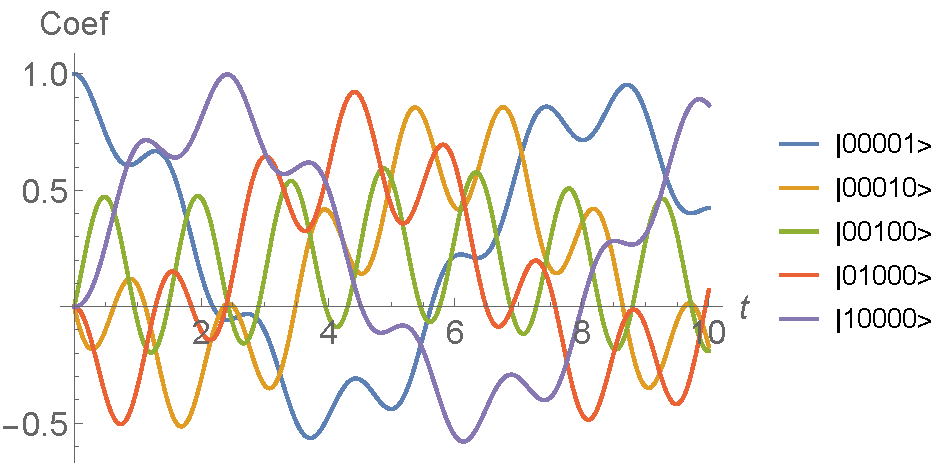
\includegraphics[width=.6\textwidth]{timeevol5dense}
	\caption{\textbf{Evolution of the 5 site system} when the system starts in state $\ket{00001}$. Periodicity is ruined by the third triplet.}
	\label{fig:timeevol5dense}
\end{figure}

\begin{figure}
	\centering
	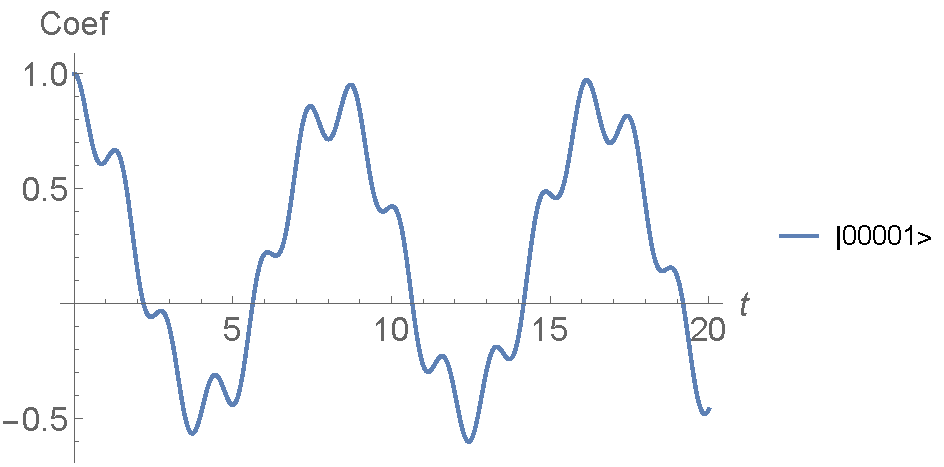
\includegraphics[width=.5\textwidth]{onecoefd}
	\caption{\textbf{Simplified view of Fig.~\ref{fig:timeevol5dense}}, showing only the coefficient for $\ket{00001}$ when that is the starting state. Even with the longer range of time, the coefficient never returns to 1.}
	\label{fig:onecoef}
\end{figure}

Instead of putting $H_3$ on every triplet, we can only chain together the odd triplets. \emph{Figure} We will call these sparse systems, and they are only possible for odd $L$. For example the sparse Hamiltonian for $L=5$ is
\begin{align}
H'_5 = H_3\otimes\mathbb{I}_2 + \mathbb{I}_2\otimes H_3.
\end{align}
Like the dense $L=5$ Hamiltonian, this system is not periodic. A plot of the coefficients over time the the starting state $\ket{00001}$ is shown in Fig.~\ref{fig:timeevol5}. An interesting detail is that the coefficient on state $\ket{00100}$ is actually periodic. 
\begin{figure}
	\centering
	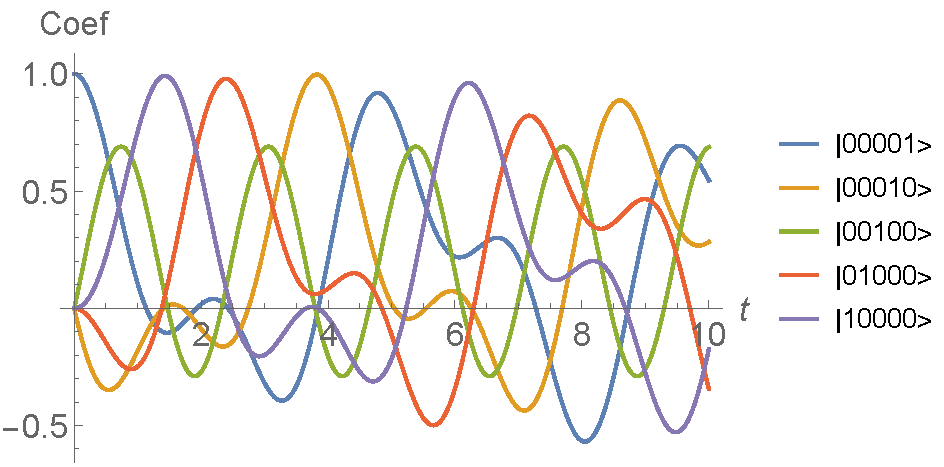
\includegraphics[width=.5\linewidth]{timeevol5}
	\caption{\textbf{Evolution of the sparse 5-site system}. Although the coefficients for most states are not periodic, the coefficient for $\ket{00100}$ is.}
	\label{fig:timeevol5}
\end{figure} 
This is the last vestige of periodicity left over from the small systems, and provides a small argument for using the dense systems, since the aperiodic systems spread more fully.

Note that the previous analysis has focused only on individual states, not operator spreading. Furthermore, for larger systems, looking at all coefficients becomes unwieldy. We can solve these problems simultaneously by using the tools developed in the previous section for quantifying operator spreading.

Before doing this, though, we will show that this Hamiltonian is quantum chaotic through an analysis of its spectrum. One method of diagnosing quantum chaos that is robust to finite size effects is the two-gap level statistics~\cite{Oganesyan2007}. From the energy eigenvalues $E_n$ define the gaps $\delta_n= E_{n+1}-E_n>0$. The level statistics are
\begin{align}
0\le r_n=\frac{\min\{\delta_n,\delta_{n-1}\}}{\max\{\delta_n,\delta_{n-1}\}}
	\le1.\label{eqn:levelstats}
\end{align}
In a random matrix the eigenvalues repel each other, so $r_n$ are not close to 0.

To calculate out level statistics we find $r_n$ and keep all but those for highest and lowest $n$. We also include a small term  
\begin{align}
H'\propto\sum_i S_i\cdot S_{i+1}
\end{align}
to break the rotational symmetry of the system. This small term does not noticeably affect any results in this section. The distribution of $r_n$ is shown in Fig.~\ref{fig:level_stats_denseL11}.
\begin{figure}
	\centering
	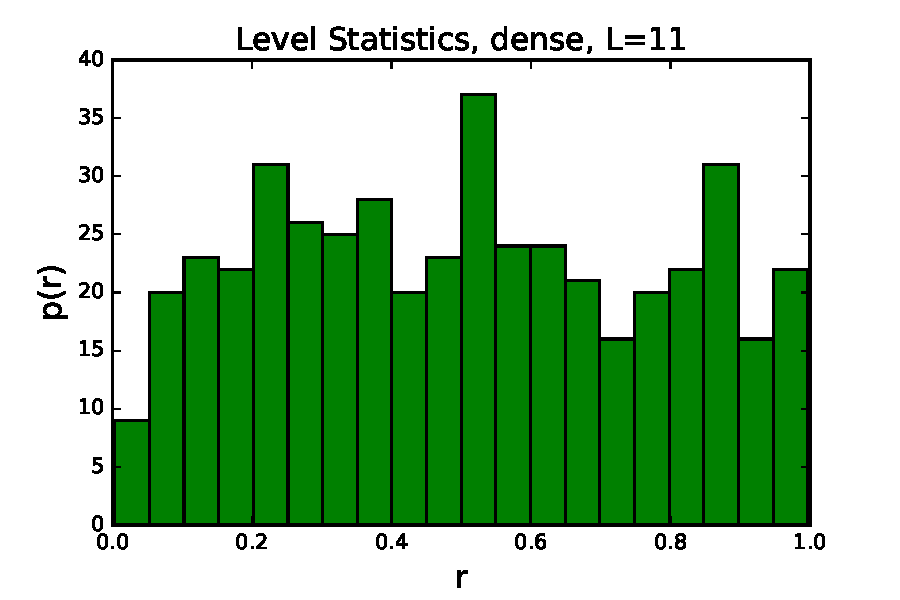
\includegraphics[width=.5\textwidth]{level_stats_denseL11}
	\caption{\textbf{Level statistics for dense Hamiltonian.}}
	\label{fig:level_stats_denseL11}
\end{figure}
The distribution does appear to be suppressed at small $r$, so we conclude that this Hamiltonian is quantum chaotic.

\subsubsection{Pauli String Weight} \label{subsub:pauli}  

We can study the operator dynamics of this system by extending to large $L$ and evolving operators that are identities on all sites except one end. The operators in this section are interpreted as observables, so they will evolve in the Heisenberg picture and cycle in the opposite direction than the states. Since the Hamiltonian is SO(3) symmetric, it does not matter if the perturbation is $X$, $Y$, or $Z$. For convenience, we will use $Z$. We start by discussing the Pauli weight, and delay discussing the OTOC and butterfly velocity to Sec.~\ref{subsub:otoc}.

The first Hamiltonian we will discuss is the $L=11$ sparse Hamiltonian. Although we will eventually use the dense one to study $v_B$, we can extract interesting behavior from the sparse one.
For the right-propagating wave, with $A(t=0) = Z_0 = Z\otimes \mathbb{I} \otimes \mathbb{I} \cdots$, the weight all starts on site 0. As it evolves, it reaches peaks for even sites, but does not rise above $1/10$ for the odd sites. The successive peaks fall off in size but dominate the Pauli strings until the last site takes over. This evolution can be seen in Fig.~\ref{fig:L11end3n20front}). 

To understand this behavior, realize that $W(i,t)$ only measures the weight of operators that end on site $i$, not those that reach past it. So, if all components of the operator that are non-identity on site $i$ are also non-identity on site $i+1$, $W(i,t)$ will be very small. Since our Hamiltonian connects site 0 with site 1 only through terms that also connect site 0 to site 2, this even-site hopping behavior makes sense. 
%Furthermore, although the Hamiltonian was designed to 

\begin{figure}
	\centering
	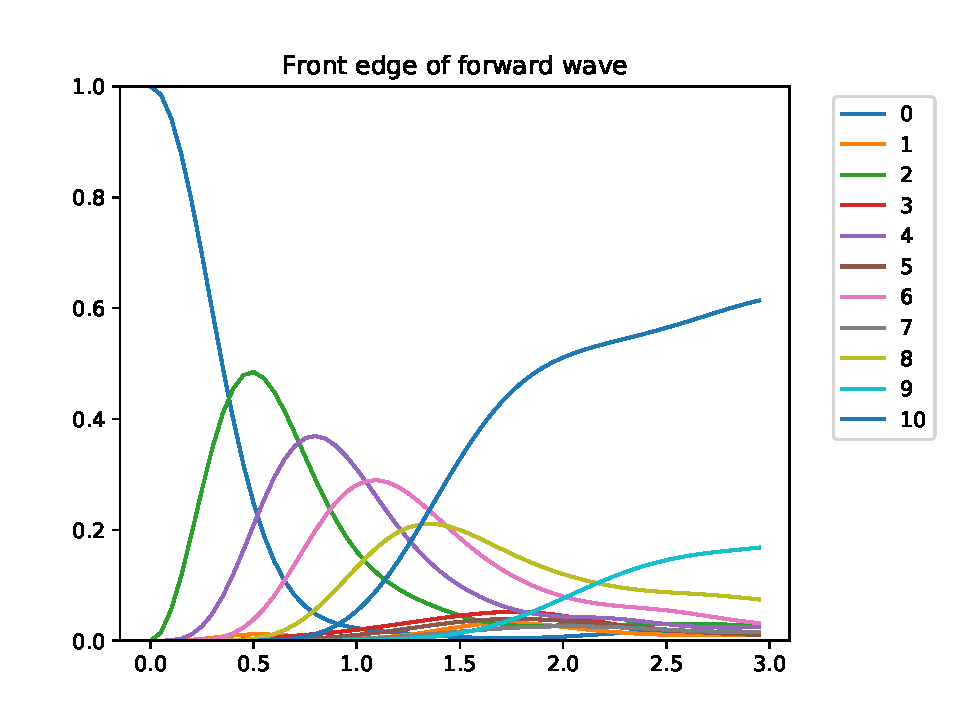
\includegraphics[width=.7\textwidth]{L11end3n20front}
	\caption{Weight of operators that end on site $i$.}
	\label{fig:L11end3n20front}
\end{figure}

For the left-propagating waves, with $A(t=0)=Z_{L-1}$, the initial decaying signal is more difficult to make out but still present. Like in the right wave, it touches only even sites. The signal travels faster and decays faster. It is dominated by a large weight of sites that start on site 9 around $t=1$. By $t = 3$ the first site has started to dominate the Pauli weights. These weights appear in Fig.~\ref{fig:L11end3n20back}.

Both the faster speed of the signal and the early dominance of the weight on site 9, which would be analogous to weight on site 1 in the right-moving case, can be understood through the asymmetric 3-site Hamiltonian and Fig.~\ref{fig:timeevol}. First recall that evolution of operators proceeds in the opposite direction as evolution of states. Then, starting on site 0, a small amount of weight would initially move to site 1 before the entire weight moves to site 2. The fact that the entire weight moves to site 2 allows the evolution in Fig.~\ref{fig:L11end1n60fore} to be so smooth. However, if the weight starts on site 10, a small amount moves to site 8 before the entire weight moves to site 9. This explains both main differences between the left and right propagating signals.

\begin{figure}
	\centering
	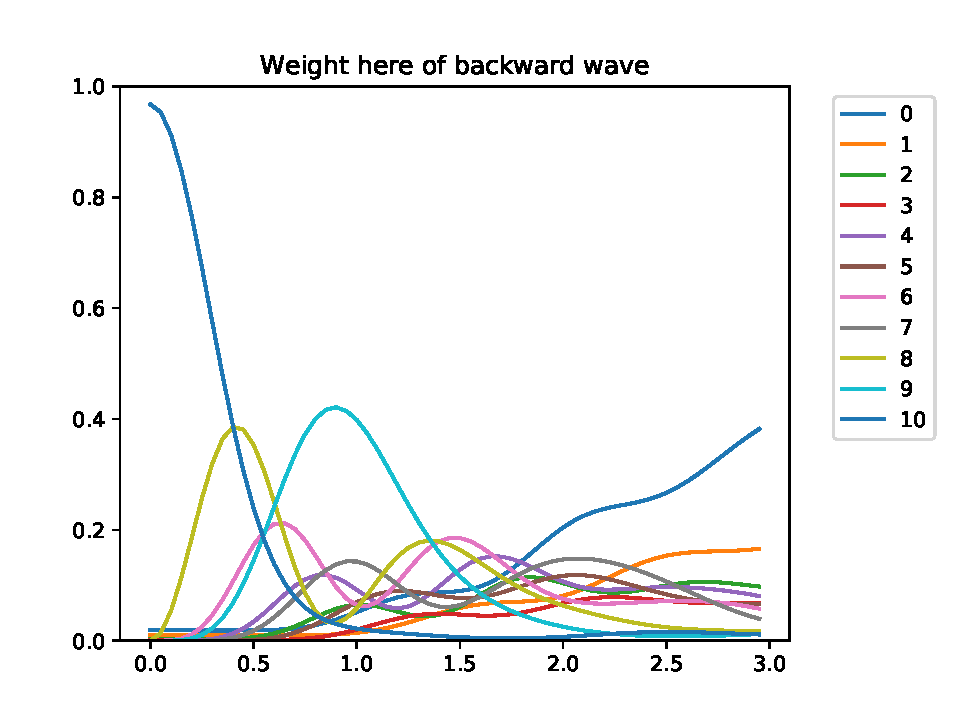
\includegraphics[width=.7\textwidth]{L11end3n20back}
	\caption{Weight of operators that begin on site $i$.}
	\label{fig:L11end3n20back}
\end{figure}

Although the long-time behavior is interesting, it is strongly affected by finite size effects and is not useful in extracting operator dynamics. For this we use the early-time behavior, in the range in which Pauli weights are still growing polynomially. For right propagation the initial behavior is $W(t;i) = \exp(a+b\log(t))=e^ab^t$ with $a,b$ given by
\begin{align*}
\begin{tabular}{rll}
$i$ & $b$ & $a$\\
0 &-0.22806104 &-0.64537868\\
1 & 3.506984  &-0.7706456\\
2 & 1.81723584  &1.24814523\\
3 & 5.61941276 &-0.85107562\\
4 & 3.84629108  &1.71062193\\
5 & 7.69020229 &-1.63644758\\
6 & 5.8674097   &1.33960991\\
7 & 9.7051822  &-2.99655938\\
8 & 7.8830393   &0.37761653\\
9 & 11.6271597   &-4.90046795\\
10 & 9.88377179 &-1.04727877
\end{tabular}
\end{align*}
The interesting data here is that the exponents are close to even integers. Even sites start with $b=0$ at site 0 and increase by 2 for each site, while odd sites start with $b=4$ at site 3. 
Figure~\ref{fig:L11end1n60fore} shows this behavior, while figure~\ref{fig:L11end1n60back} shows the analogous behavior for the left propagating wave. The exponents there follow a similar pattern.

\begin{figure}
	\centering
	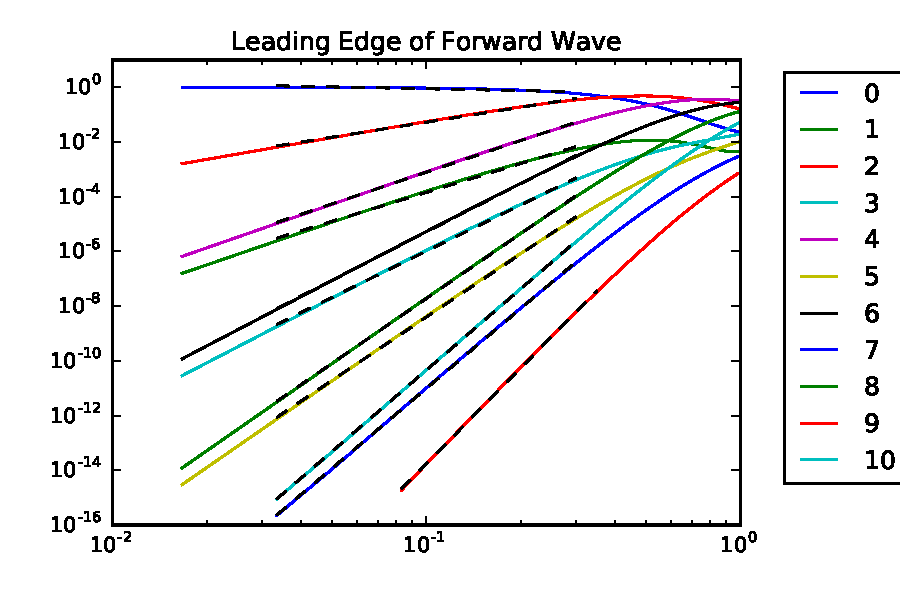
\includegraphics[width=.7\textwidth]{L11end1n60fore}
	\caption{Early-time leading edge weights for right propagating wave.}
	\label{fig:L11end1n60fore}
\end{figure}
\begin{figure}
	\centering
	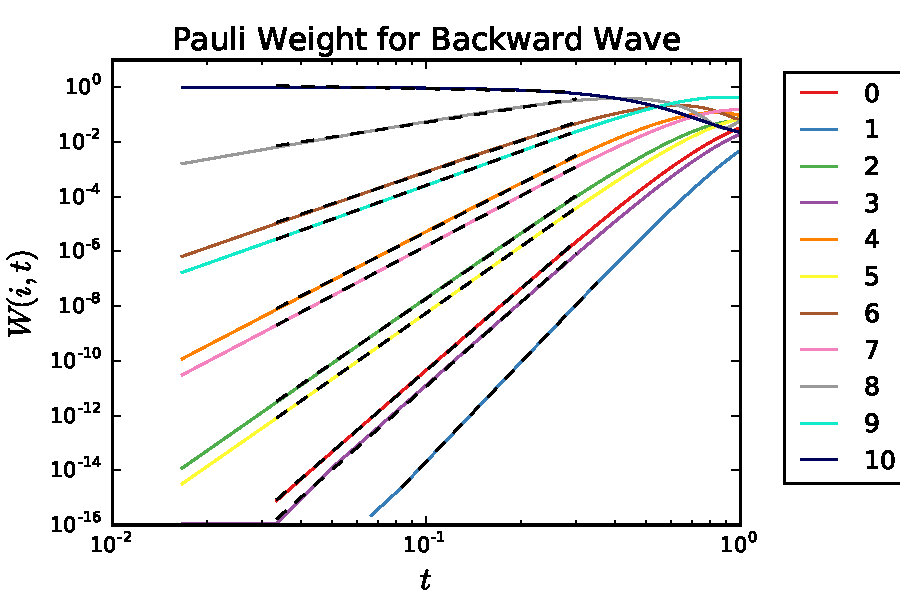
\includegraphics[width=.7\textwidth]{L11end1n60back}
	\caption{Early-time leading edge weights for left propagating wave.}
	\label{fig:L11end1n60back}
\end{figure}

To understand these exponents, treat $t$ in the time evolution operator as a perturbation,
\begin{align}
U(t) &= e^{iHt}\nn
&= 1-iHt-\half H^2t^2+\frac{i}{3!}H^3+\th{4!}H^4t^4+\dots\label{eqn:expansion}
\end{align}
The term linear in $t$ contains a single $H$, which has matrix elements that connect site 0 to sites 1 and 2. The term quadratic in $t$ contains a second $H$, which connects site 0 to sites 3 and 4 through site 2. The Pauli weight is quadratic in $A(t)$, which explains why the exponents for the OTOC are even.

Although this explains why the exponents for even sites are $0,2,4\dots$, it suggests that the exponents for odd sites should be $2,4,6\dots$. The reason they are not is the same reason that the weight on these sites is suppressed in the full evolution: they are hidden to first available order by the sites in front of them. To see the $t^2$ dependence on site $1$, for example, we need the weight of all operators that are non-zero at that site, not just the ones that end there. We can find this information in $C(i,t)$, the normalized OTOC.

\subsubsection{OTOC and Butterfly Velocity} \label{subsub:otoc}

After discussing the behavior of the Pauli weights in the sparse and dense Hamiltonians, we will discuss the OTOC, which encodes the amount of operator weight on a site, and from this explore the butterfly velocity. We do not find an explicit $v_B$ but do show that it is different in the two directions. 

First we show the full time evolution of the OTOC for the sparse and dense Hamiltonians, for left and right propagating waves. These can be found in Figs.~\ref{fig:L11end3n20_herefront} through~\ref{fig:denseL11end3n20_hereback}. The most most obvious difference from the Pauli weight is that these weights asymptote to a non-zero value for all sites. As discussed in Eq.~\ref{eqn:otoc} the OTOC measures the weight of non-identity operators on a site, and asymptotes to $1/2$ in random matrices, or $3/4$ in our normalization. The operators in this Hamiltonian do not reach $3/4$ because of their conservation laws~\cite{Jonay17, Jonay18}.

Other interesting features include the persistence of the fast-moving signal in the left-moving wave of the sparse Hamiltonian and the clear asymmetry in early behavior between left- and right-moving OTOCs. The OTOCs for perturbations starting on site 0 consistently rise faster than the signals propagating from site 10. The dense Hamiltonian also transports weight faster than the sparse Hamiltonian.

\begin{figure}
	\centering
	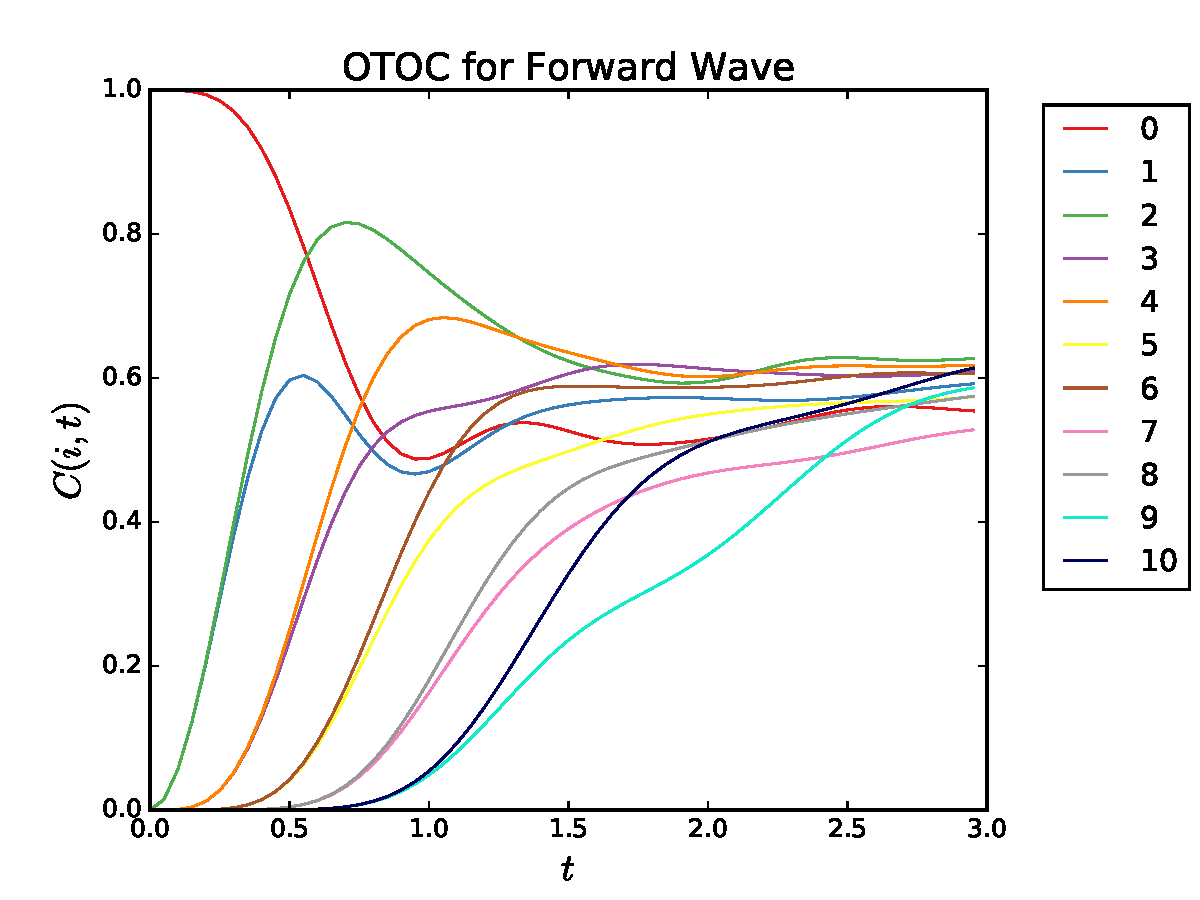
\includegraphics[width=.7\textwidth]{L11end3n20_herefront}
	\caption{\textbf{OTOC for sparse Hamiltonian,} right moving perturbation.}
	\label{fig:L11end3n20_herefront}
\end{figure}

\begin{figure}
	\centering
	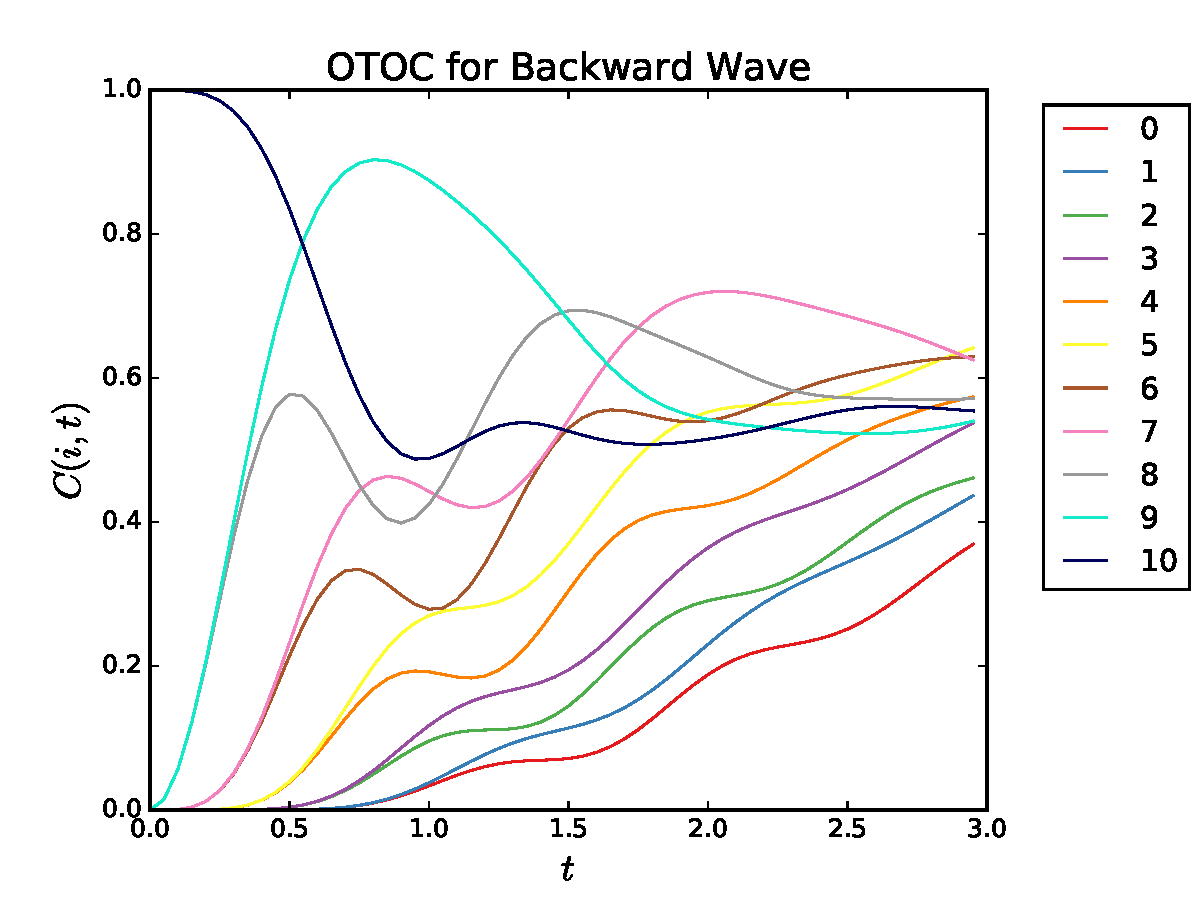
\includegraphics[width=.7\textwidth]{L11end3n20_hereback}
	\caption{\textbf{OTOC for sparse Hamiltonian,} left moving perturbation.}
	\label{fig:L11end3n20_hereback}
\end{figure}

\begin{figure}
	\centering
	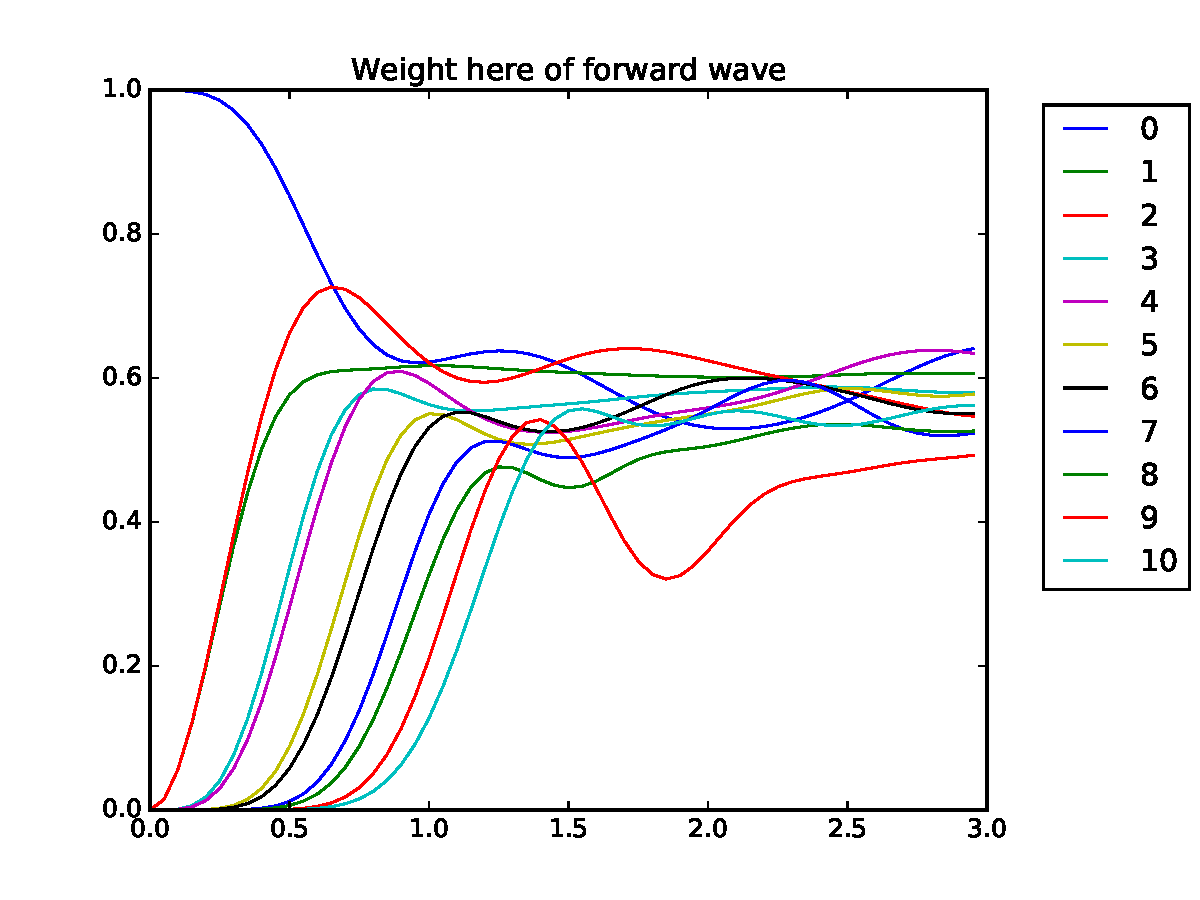
\includegraphics[width=.7\textwidth]{denseL11end3n20_herefront}
	\caption{\textbf{OTOC for dense Hamiltonian,} right moving perturbation.}
	\label{fig:denseL11end3n20_herefront}
\end{figure}

\begin{figure}
	\centering
	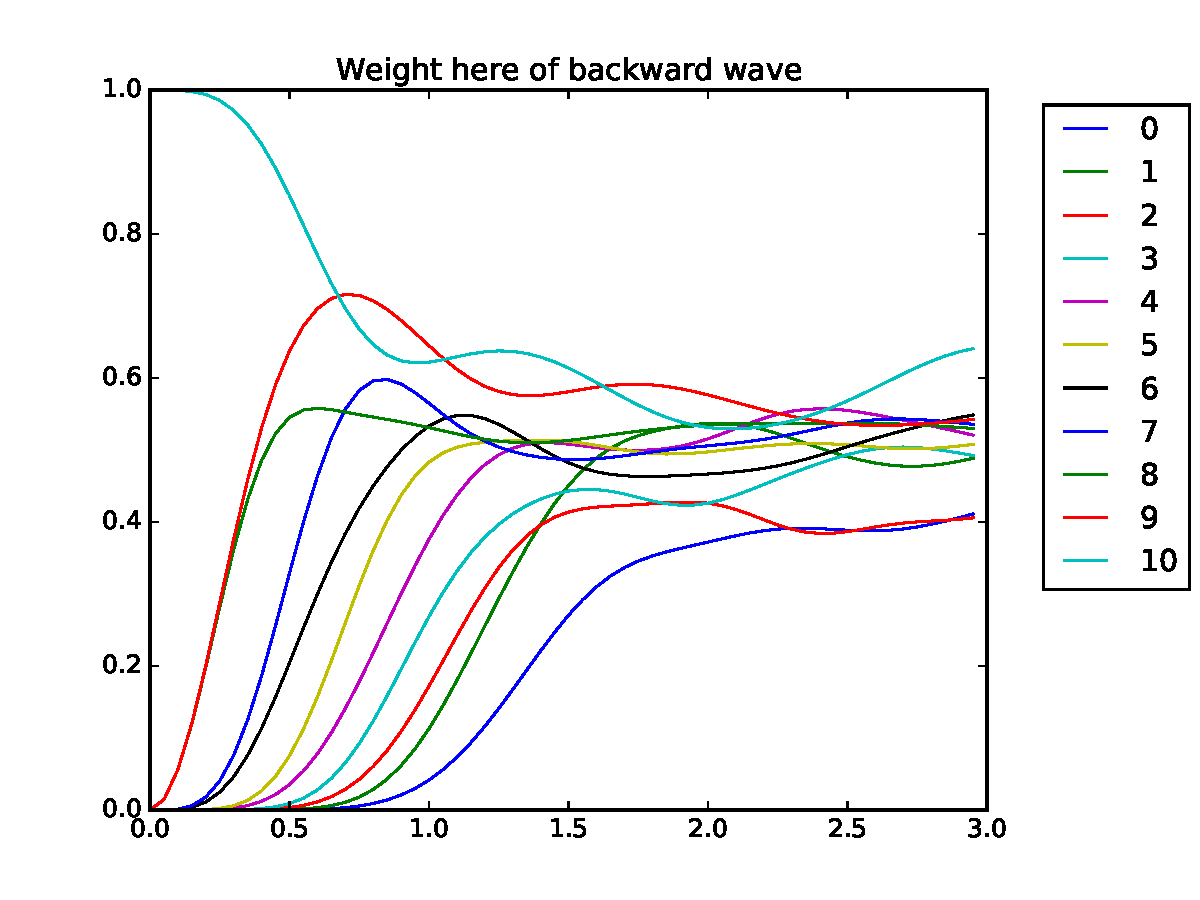
\includegraphics[width=.7\textwidth]{denseL11end3n20_hereback}
	\caption{\textbf{OTOC for dense Hamiltonian,} left moving perturbation.}
	\label{fig:denseL11end3n20_hereback}
\end{figure}

Like for the Pauli weights we can study the early behavior. We will only show the plot for for the forward wave for the sparse Hamiltonian, \emph{Why?}

To find the butterfly velocity, we have to first find the velocity-dependent Lyapunov exponents $\lambda(v)$. To do this we plot $C(vt,t)$, where $vt=i$, for different values of $v$. For a sufficiently large system there should be a $v=v_B$ such that $C(vt,t)$ does not decay with $t$. Our system suffers from finite size effect that prevent us from finding $v_B$ exactly, but we can still explore the $v$ dependence of $C(vt,t)$.

We will focus on the dense Hamiltonian, as it has more asymmetry. Unsurprisingly, $C(vt,t)$ suffers from the same odd/even effects we've been seeing all along. Fig.~\ref{fig:otocs_denseforeallL11} shows the evolution of the weights. The problem is that weight too quickly reaches the even sites and does not reach the odd sites fast enough.

\begin{figure}
	\centering
	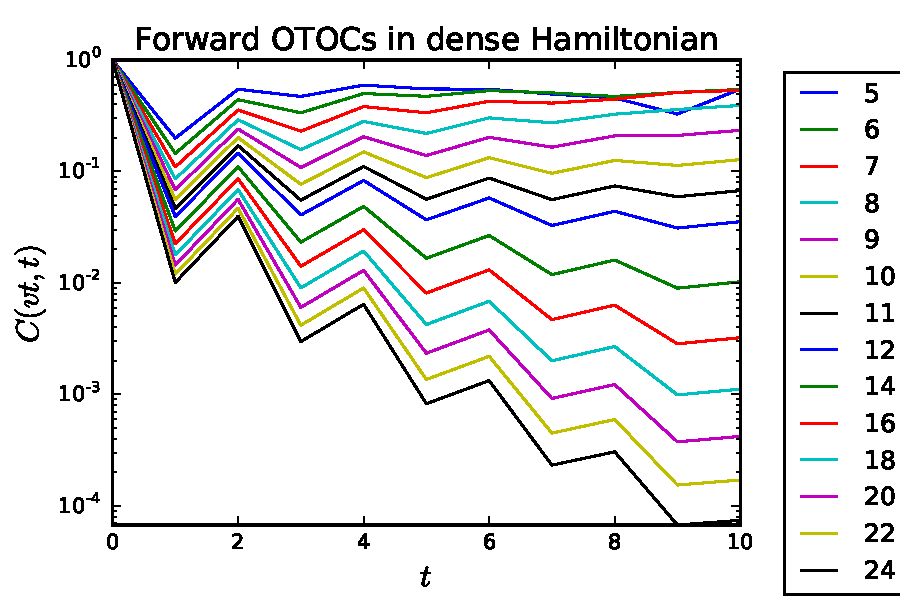
\includegraphics[width=.495\textwidth]{otocs_denseforeallL11}
	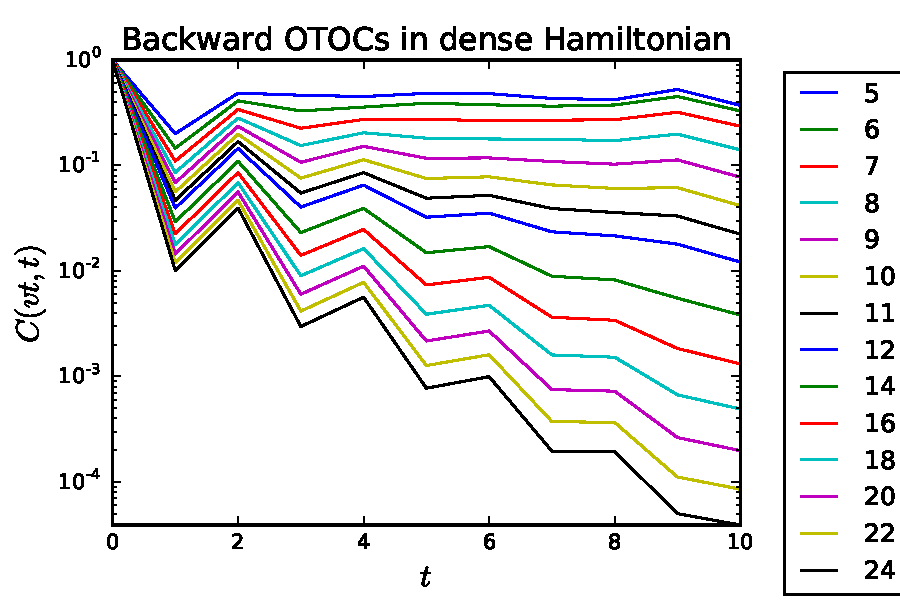
\includegraphics[width=.495\textwidth]{otocs_densebackallL11}
	\caption{\textbf{Velocity-dependent OTOC decay} in dense Hamiltonian. The jaggedness comes from odd/even effects. Each line corresponds to a velocity, given in the legend. The overall behavior is exponential decay as expected.}
	\label{fig:otocs_denseforeallL11}
\end{figure}

We could still use these plots to calculate $\lambda(v)$, but there are few enough sites that the calculation will have high uncertainty. Alternatively we can boost the odd sites by connecting site 0 to site 1 with a term that does not connect it to site 2. This will change the overall dynamics but hopefully only by bringing neighboring sites closer to each other, so that it does not change the dynamics averaged over even and odd sites.

The simplest rotationally symmetric term with the desired property is $H'=\bm{S}_i\cdot\bm{S}_j$. The coefficient of $H'$ should be chosen to maximize the smoothness of the OTOC. Empirically, a very effective coefficient is 4. Smaller constants left too much of the jaggedness, and larger constants introduced jaggedness in the other direction. We also dd a 2-site term to spins 9 and 10, to have the same effect on the backwards wave. The total Hamiltonian is
\begin{align}
H = \frac{2\pi}{3\sqrt{3}}\sum_{i=0}^{L-2}\bm{S}_i \cdot \left(\bm{S}_{i+1}
	\times\bm{S}_{i+2}\right) + 4\left(\bm{S}_0\cdot\bm{S}_1 + \bm{S}_{L-2}
	\cdot\bm{S}_{L-1}\right).
\end{align}
This perturbation is large enough to noticeably change the plots of the Pauli weight and the OTOC, by shuffling weight back and forth between the initial two sites early in the evolution. However the early time behavior, averaged over even and odd sites, is similar enough to not change $\lambda(v)$ dramatically.

Using the new Hamiltonian, the OTOC decay becomes much more linear, although still not perfectly so, as shown in Fig.~\ref{fig:otocs_pert}.
\begin{figure}
	\centering
	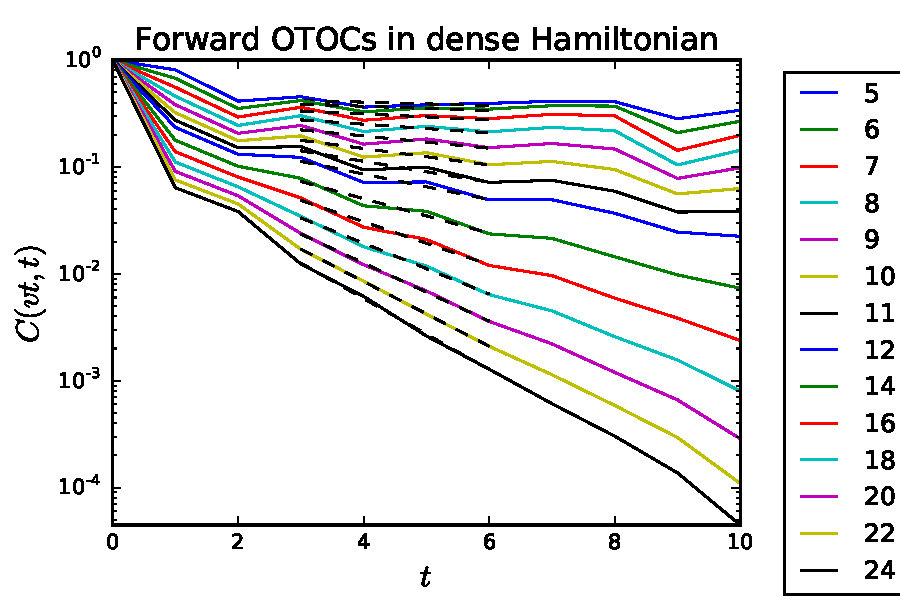
\includegraphics[width=.495\textwidth]{otocs_dense_pert_foreallL11}
	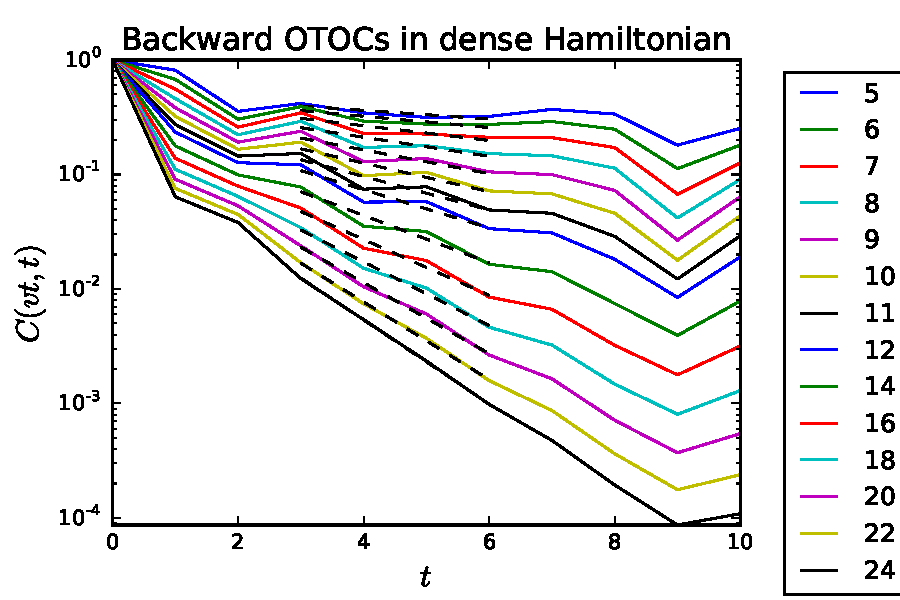
\includegraphics[width=.495\textwidth]{otocs_dense_pert_backallL11}
	\caption{\textbf{Velocity-dependent OTOC decay} in dense Hamiltonian with initial and final dot product perturbations. Although there is still jaggedness on the edges, the linear behavior in the bulk allows us to extract $\lambda(v)$.}
	\label{fig:otocs_pert}
\end{figure}
Fig.~\ref{fig:balanced_butterfly_dense_pert_L11} shows the $v$ dependence of $\lambda(v)$. In a large enough system, $\lambda(v)$ should approach 0 for finite $v$. However, due to the small size of our system we were not able to effectively probe these slow speeds. However, it is clear that $\lambda_+>\lambda_-$ for all $v$. Therefore, for these time-independent Hamiltonian systems, $v_{B+}>v_{B-}$.
\begin{figure}
	\centering
	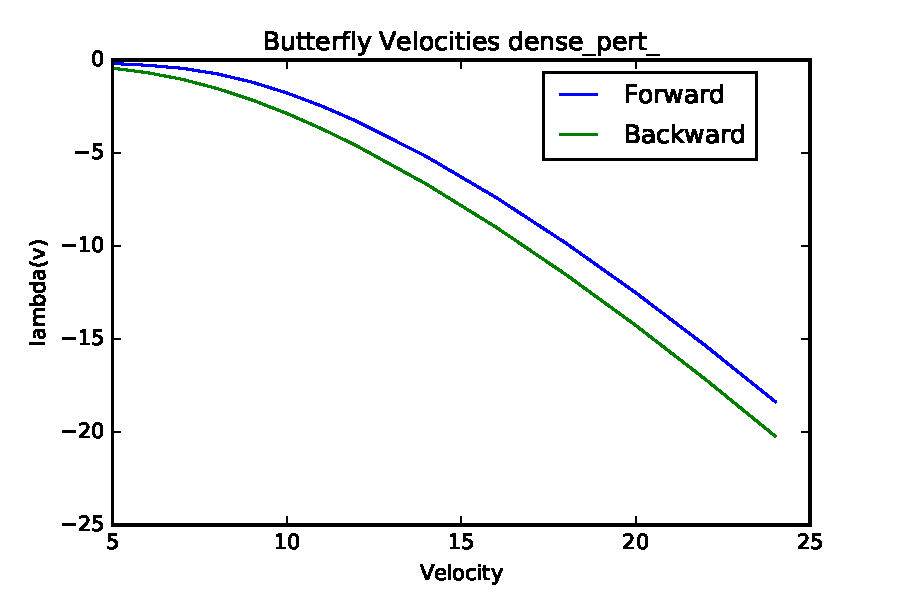
\includegraphics[width=.5\textwidth]{balanced_butterfly_dense_pert_L11}
	\caption{\textbf{Velocity dependent Lyapunov exponents} for the dense Hamiltonian with end perturbations. The butterfly velocity should be where these curves cross the origin, such $\lambda(v_B) = 0$. This doesn't happen, due to finite size effects, but we can see that $\lambda_+>\lambda_-$ for all $v$, which implies that $v_{B+}>v_{B-}$.}
	\label{fig:balanced_butterfly_dense_pert_L11}
\end{figure}